% Settings for the default beamer theme
\documentclass[english, aspectratio=169]{beamer}
\usepackage[T1]{fontenc}
\usepackage[utf8]{inputenc}
\usepackage{tabularx}
\usepackage{babel}
\usepackage[ruled,vlined]{algorithm2e}
\SetAlgorithmName{Algoritmus}{algoritmus}{List of Algorithms}
\setcounter{secnumdepth}{3}
\setcounter{tocdepth}{3}

\makeatletter

\newcommand\makebeamertitle{\frame{\maketitle}}

% (ERT) argument for the TOC
\AtBeginDocument{%
  \let\origtableofcontents=\tableofcontents
  \def\tableofcontents{\@ifnextchar[{\origtableofcontents}{\gobbletableofcontents}}
  \def\gobbletableofcontents#1{\origtableofcontents}
}

% Theme settings
\usetheme{Frankfurt}
\usecolortheme{default}
\usefonttheme[onlymath]{serif}

% Template settings
\setbeamertemplate{navigation symbols}{}
\setbeamertemplate{blocks}[rounded][shadow=false]
\setbeamertemplate{title page}[default][colsep=-4bp, rounded=true, shadow=false]
\makeatother

\begin{document}

% Title page
\section{Bevezetés}
\title[]{Üzleti Intelligencia}
\subtitle{6. Előadás: Mély $Q$-tanulási architektúrák}
\author[Kuknyó Dániel]{Kuknyó Dániel\\Budapesti Gazdasági Egyetem}
\date{2023/24\\1.félév}
\makebeamertitle

% Table of contents slide
\begin{frame}
\tableofcontents{}
\end{frame}

% Table of contents of the current section
\begin{frame}
\tableofcontents[currentsection]
\end{frame}

\begin{frame}{A $Q$-tanulás alapjai}
\begin{columns}
\begin{column}{.75\textwidth}
A megerősítéses tanulásban az egyik nagy áttörést egy politikafüggetlen TD algoritmus kifejlesztése hozta el.\par\smallskip
Ebben az esetben a becsült \textbf{állapot-cselekvés minőség függvény}, $Q$, ami megadja, hogy mennyire jövedelmező az ügynöknek $s$ állapotban $a$ cselekvést végrehajtani.
\begin{block}{$Q$-érték frissítése}
\[
Q(s,a) \leftarrow Q(s,a) + \alpha \left[ r + \gamma \underset{a'}{max}Q(s',a') - Q(s,a) \right]
\]
\end{block}
A $Q$-tanulás ezáltal egy teljesen online tanulási algoritmus, ami a követett \textbf{politikától függetlenül} garantáltan konvergálni fog a valós $Q$ értékekhez.
\end{column}
\begin{column}{.25\textwidth}
\begin{center}
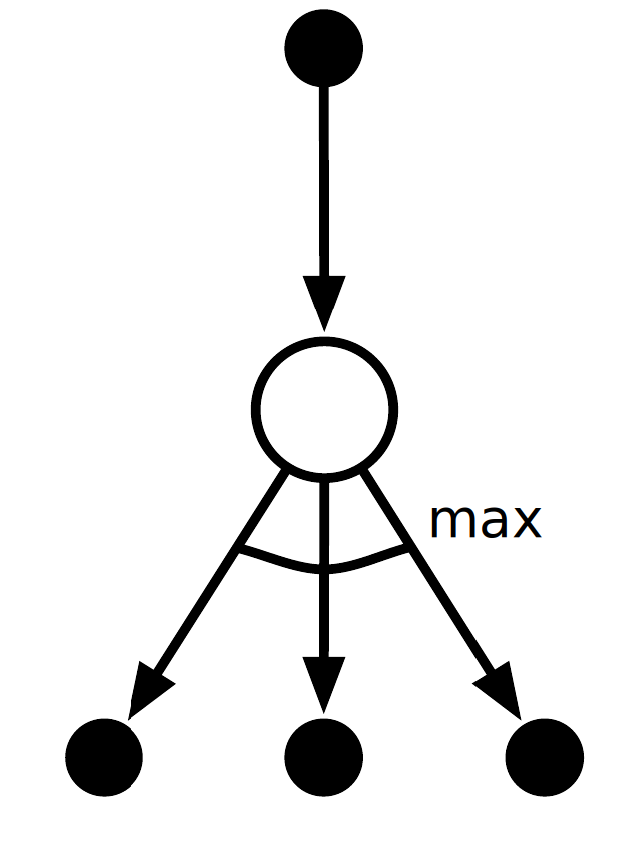
\includegraphics[width=3cm, keepaspectratio]{../../5_ql/doc/images/ql_2.png}
\end{center}
\end{column}
\end{columns}
\end{frame}

\begin{frame}{Dupla $Q$-tanulás}
A kettős tanulás ötlete kiterjed a teljes MDP algoritmusaira. A $Q$-tanulásban a becsült $Q$-értékek torzítottak lehetnek, ha alacsony a minta számossága, vagy zaj van a rendszerben. Egy módja a $Q$-tanulás regularizálásának, ha egy helyet\textbf{ két $Q$-táblát tart nyilván az algoritmus}, $Q_1$-et és $Q_2$-t.\par\smallskip
A $Q$-tanulással analóg dupla $Q$-tanulás nevű kettős tanulási algoritmus két részre osztja az időlépéseket, minden lépésben $50\%$ valószínűséggel a frissítés a következő:
\begin{block}{}
\[
Q_1(s,a) \leftarrow Q_1(s,a) + \alpha \left[ r + \gamma Q_2\left(s', \underset{a'}{argmax} Q_1(s',a')\right) - Q_1(s, a) \right]
\]
\end{block}
A többi esetben $Q_1$ és $Q_2$ felcserélésével történik, így $Q_2$ frissül. A két táblát teljesen szimmetrikusan kezeli az algoritmus. Például egy $\varepsilon$-mohó politika a dupla tanulás esetében az egyes cselekvési értékbecslések \textbf{átlagára vagy összegére épülhet}.
\end{frame}

\begin{frame}{Alapvető $Q$-tanulási eljárások}
\begin{columns}
\begin{column}{.5\textwidth}
\begin{center}
$Q$-tanulás\par\smallskip
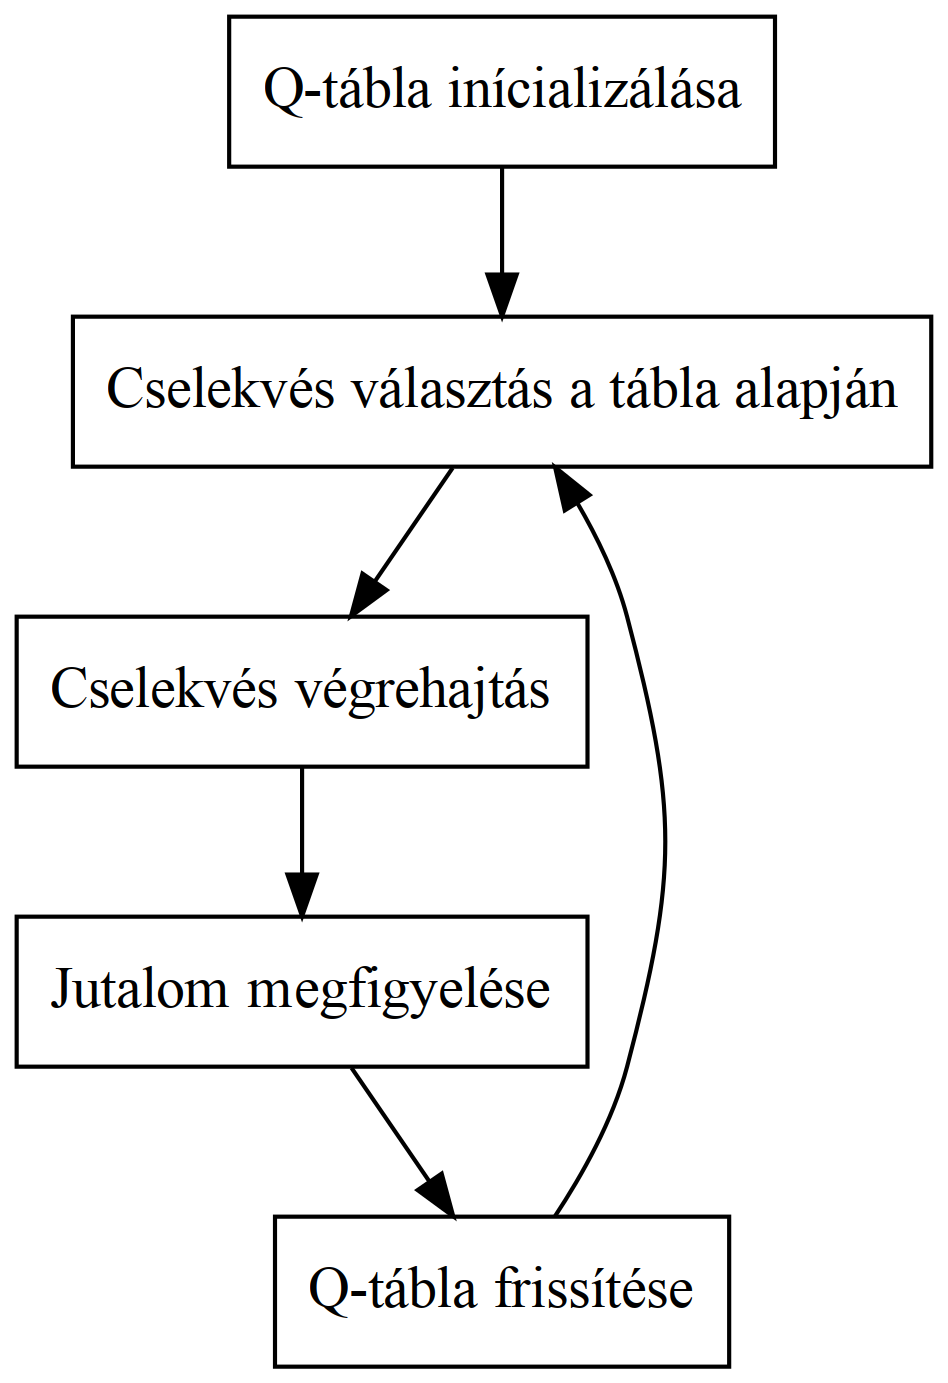
\includegraphics[height=6cm, keepaspectratio]{../../5_ql/doc/graphs/ql_1.png}
\end{center}
\end{column}
\begin{column}{.5\textwidth}
\begin{center}
Dupla $Q$-tanulás\par\smallskip
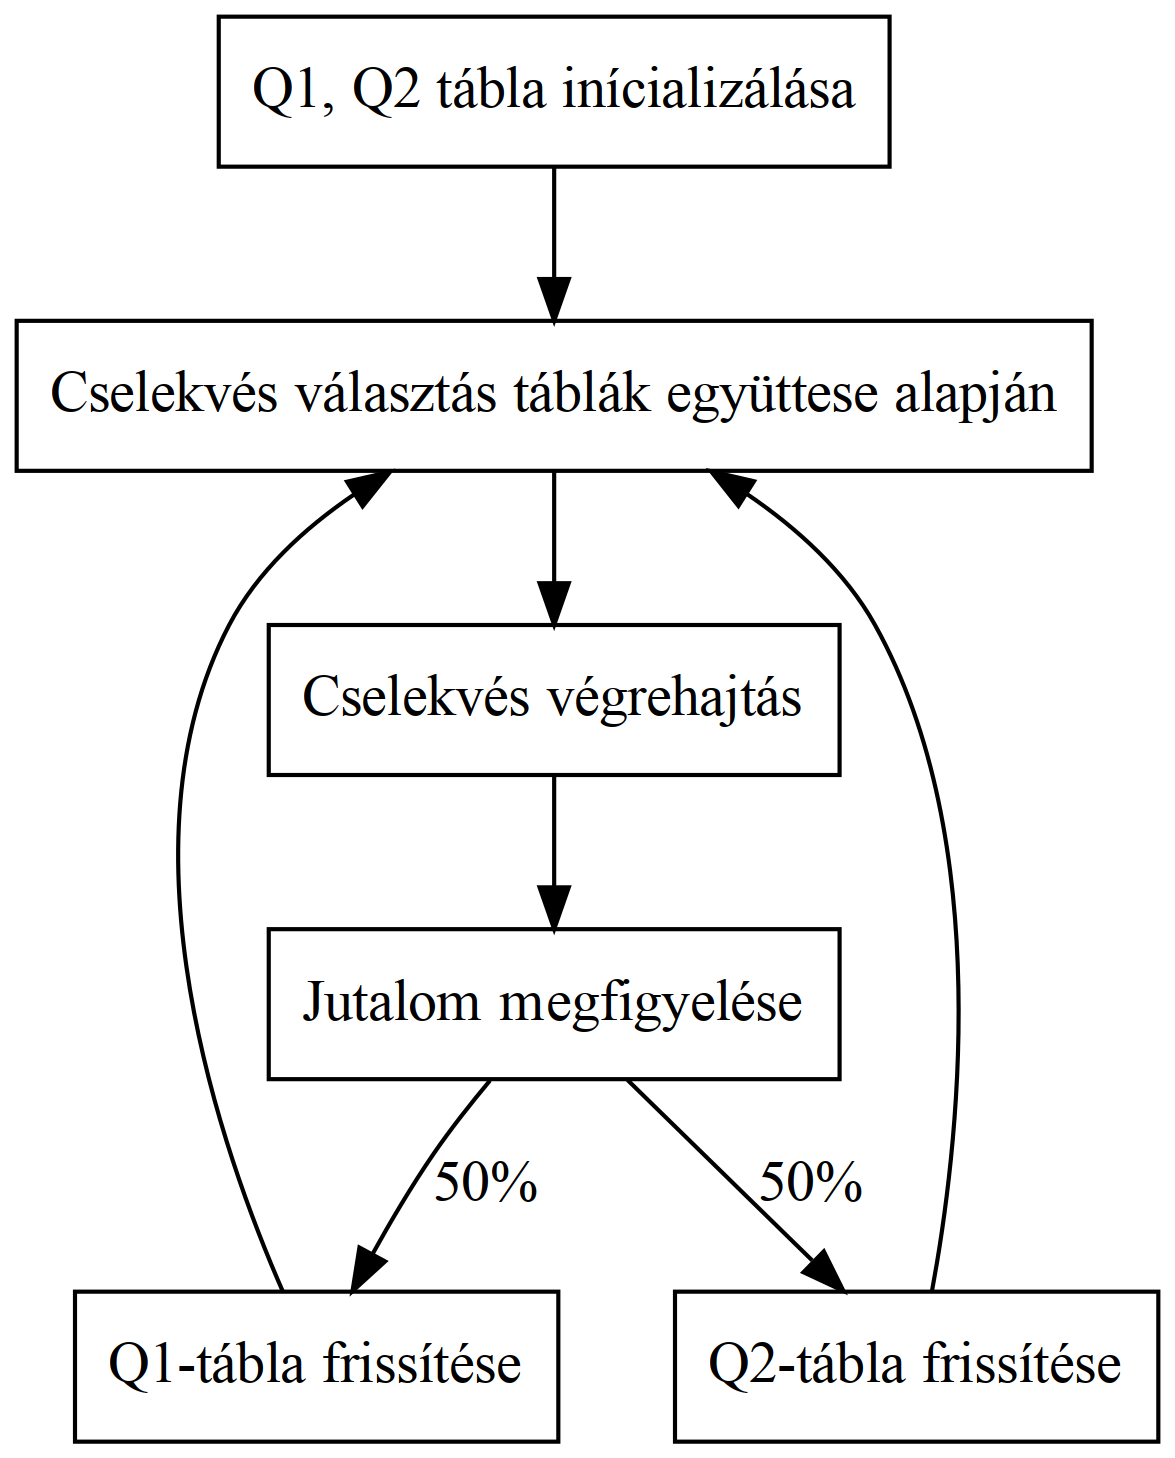
\includegraphics[height=6cm, keepaspectratio]{../../5_ql/doc/graphs/ql_2.png}
\end{center}
\end{column}
\end{columns}
\end{frame}

\section{Mély $Q$-tanulás (DQN)}

\begin{frame}
\tableofcontents[currentsection]
\end{frame}

\begin{frame}{A $Q$-hálózat (DQN)}
\begin{columns}
\begin{column}{.6\textwidth}
A $Q$-hálózat egy természetes kiterjesztése a hagyományos $Q$-tanulásnak. A naív $Q$-hálózat inputja a \textbf{környezetet leíró változók} vektora vagy mátrixa, és az outputja pedig az ügynök számára elérhető \textbf{cselekvések $Q(s,a)$ értéke} minden $a_1,a_2,..,a_n$ cselekvéshez tartozóan. \par\smallskip
A cselekvés választáshoz az ügynök kiválasztja a \textbf{legnagyobb becsült $Q$ értéket}, és az ahhoz tartozó cselekvést fogja végrehajtani.\par\smallskip
A $Q$-hálózat költségfüggvénye az \textbf{átlagos négyzetes Bellman hiba}, a paraméter frissítése pedig a költségfüggvény gradiense és a lépésméret szerint történik. 
\end{column}
\begin{column}{.4\textwidth}
\begin{center}
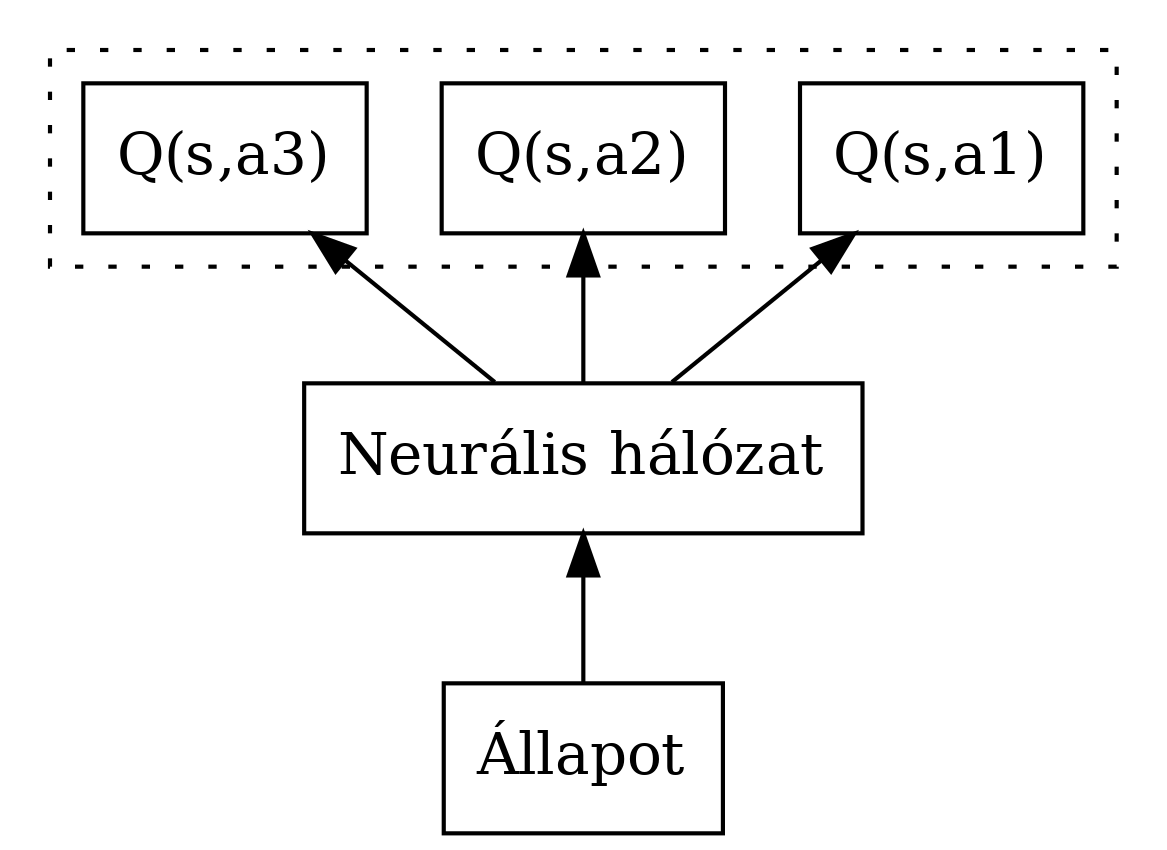
\includegraphics[width=6cm, keepaspectratio]{../../5_ql/doc/graphs/ql_3.png}
\end{center}
\end{column}
\end{columns}
\end{frame}

\begin{frame}{A DQN költségfüggvénye}
\begin{columns}
\begin{column}{.75\textwidth}
A mély $Q$-tanulás során a költségfüggvény \textbf{a négyzetes Bellman hiba várható értéke}:
\begin{block}{}
\vspace{-0.5cm}
\[
J(\theta) = E_{s,a,r,s' \sim D} \left[ \left( r + \gamma \underset{a'}{max} Q_\theta(s',a') - Q_\theta(s,a) \right)^2 \right]
\]
\end{block}	
Ahol $s,a,r,s'$ a $D$ tapasztalat visszajátszási memóriából vett minta. A $Q$-hálózat megkeresi az $s'$ következő állapothoz tartozó legnagyobb értékű cselekvést, $a'$-t, és lekérdezi a memóriából vett $s$ aktuális állapothoz és $a$ aktuális cselekvéshez tartozó $Q$-értéket. Ez a TD hibának egy változata.  
\end{column}
\begin{column}{.25\textwidth}
\begin{center}
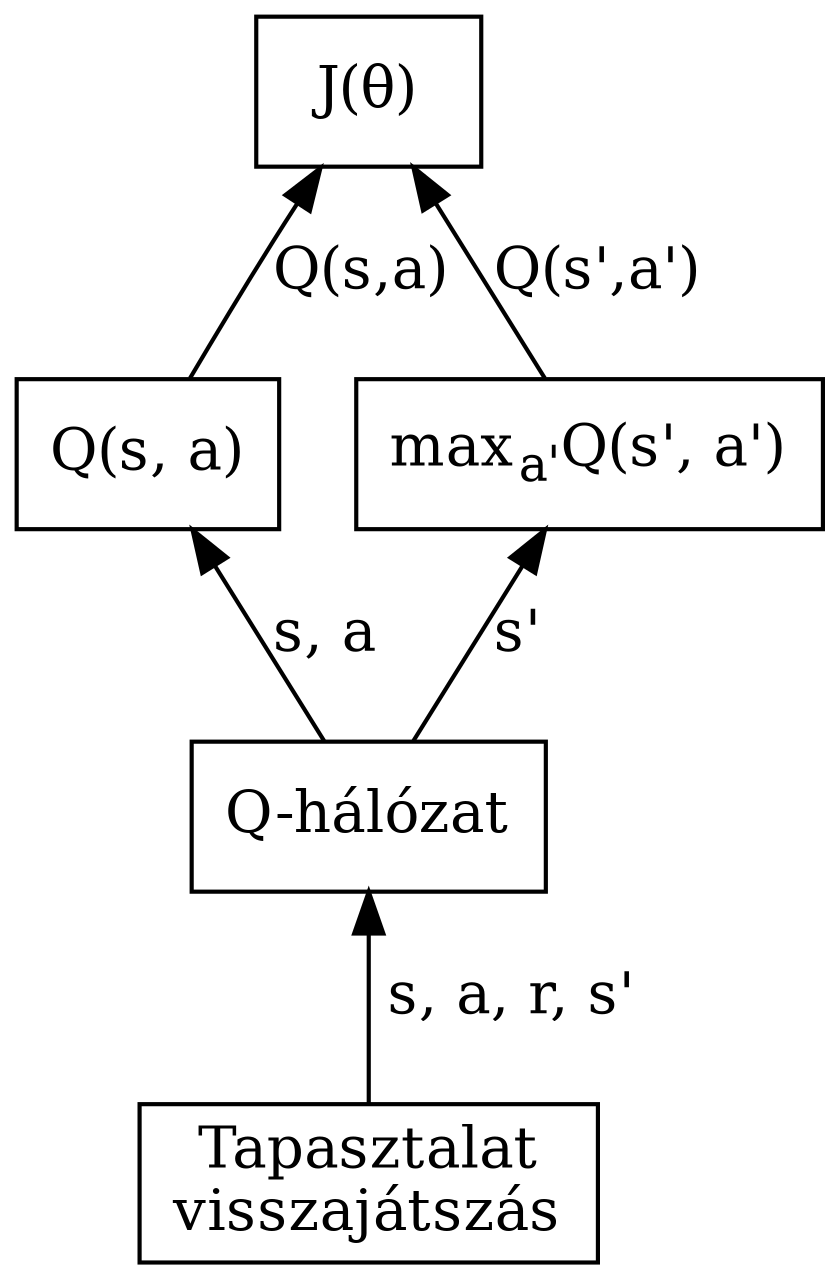
\includegraphics[height=6cm, keepaspectratio]{graphs/dql_1.png}
\end{center}
\end{column}
\end{columns}
\end{frame}

\begin{frame}{Tapasztalat visszajátszás}
\begin{columns}
\begin{column}{.65\textwidth}
A tapasztalat visszajátszás az egyik változtatás, ami a $Q$-hálózat problémáján hivatott segíteni.\par\smallskip
A tapasztalat memória ($D_{replay}$) \textbf{$[s,a,r,s']$ négyeseket tartalmaz}. Minden alkalommal amikor az ügynök cselekszik, az általa tapasztalt $s, a, r, s'$ elmentődik a tapasztalat memóriába.\par\smallskip
Amikor tanulásra kerül a sor, az ügynök \textbf{véletlen és rendezetlen mintát} (miniköteget) kap a tapasztalat memóriából, melynek számossága megegyezik a kötegmérettel. Eszerint számolódik ki a költségfüggvény majd frissülnek a $Q$-hálózat paraméterei.
\end{column}
\begin{column}{.35\textwidth}
\begin{center}
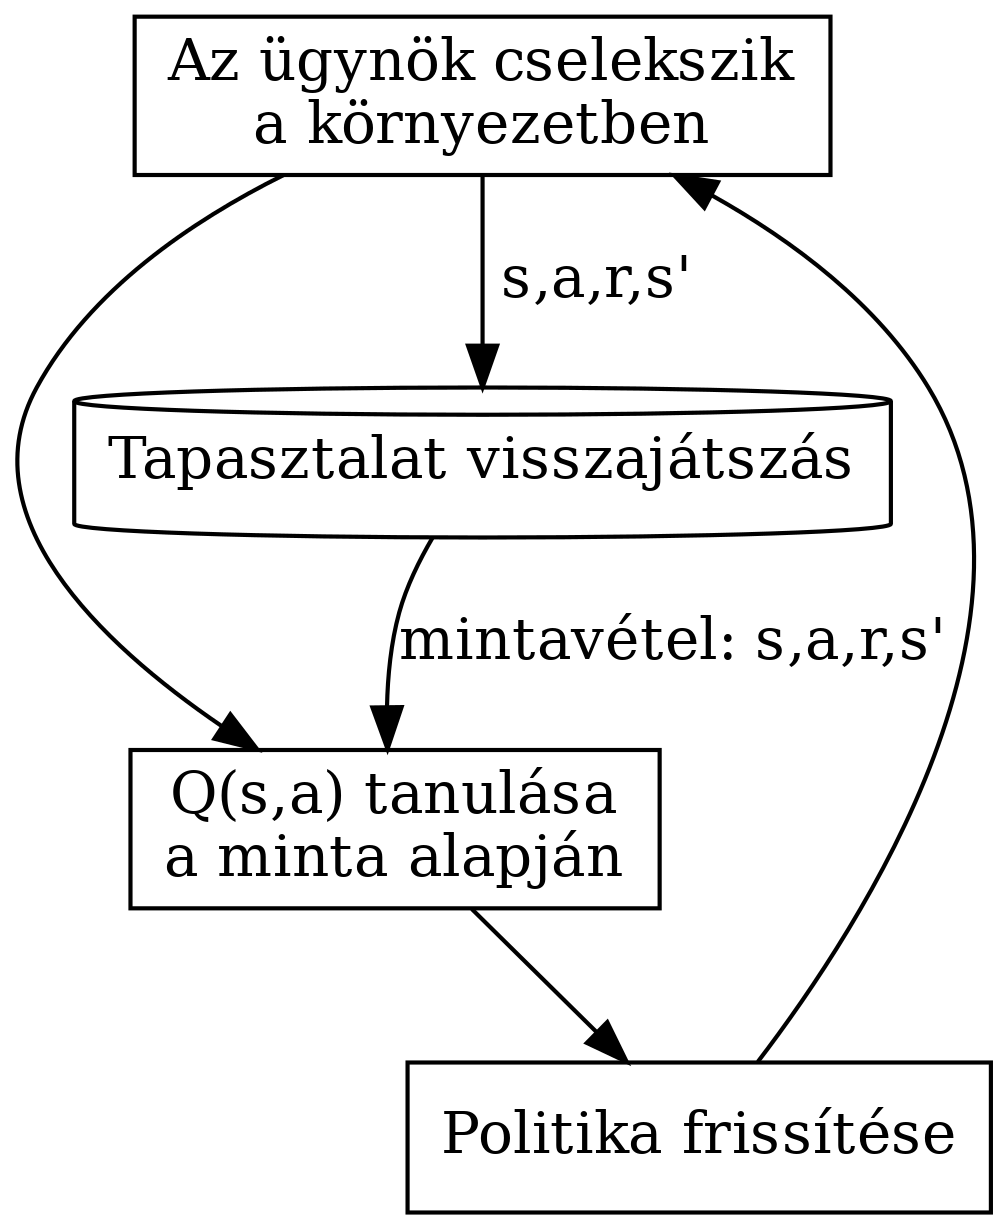
\includegraphics[height=6cm, keepaspectratio]{../../5_ql/doc/graphs/ql_4.png}
\end{center}
\end{column}
\end{columns}
\end{frame}

\begin{frame}{}
\begin{algorithm}[H]
\caption{Mély $Q$-tanulás}
\SetAlgoLined
$Q$-hálózat $Q_\theta$ inicializálása, tapasztalat memória $D$ inicializálása\;
\For{$i = 0 \rightarrow max_i$}{
	\For{$t = 0 \rightarrow max_t$}{
		$s$ megfigyelése és $a \sim \pi(s,a)$ cselekvés választása\;
		$a$ végrehajtása és $s'$, $r$ megfigyelése\;
		$s, a, r, s'$ eltárolása a tapasztalat memóriában\;
	}
	\For{$c = 0 \rightarrow max_c$}{
		$e = s, a, r, s' \sim D$\tcc*[t]{Mintavétel a tapasztalat memóriából}
		Gradiens ereszkedés végrehajtása $\left( r + \gamma \underset{a'}{max}Q_\theta(s',a') - Q_\theta(s,a) \right)^2$ hibán\;
	}		
}
\end{algorithm}
Ahol $t$ a környezetben lejátszott lépések és $c$ a hálózat tanítási lépések ciklusváltozója.
\end{frame}

\section{Dupla mély $Q$-tanulás (DDQN)}

\begin{frame}
\tableofcontents[currentsection]
\end{frame}

\begin{frame}{DDQN}
\begin{columns}
\begin{column}{.5\textwidth}
A DDQN algoritmusa a dupla $Q$-tanulás elveit hajtja végre neurális hálózatokkal: ebben az esetben a két $Q$-tábla helyett \textbf{két $Q$-hálózat} kap helyet az architektúrában:
\begin{itemize}
	\item Online hálózat $Q_\theta$: a cselekvések \textbf{kiválasztásáért} felel.
	\item Célhálózat $Q_{\bar{\theta}}$: a választott cselekvés \textbf{kiértékeléséért} felel.
\end{itemize}
Az algoritmus csak az online hálózaton hajt végre paraméter frissítést. A célhálózatot úgy frissíti, hogy az online hálózat paramétereinek értékét átmásolja adott időközönként. 
\end{column}
\begin{column}{.5\textwidth}
\begin{center}
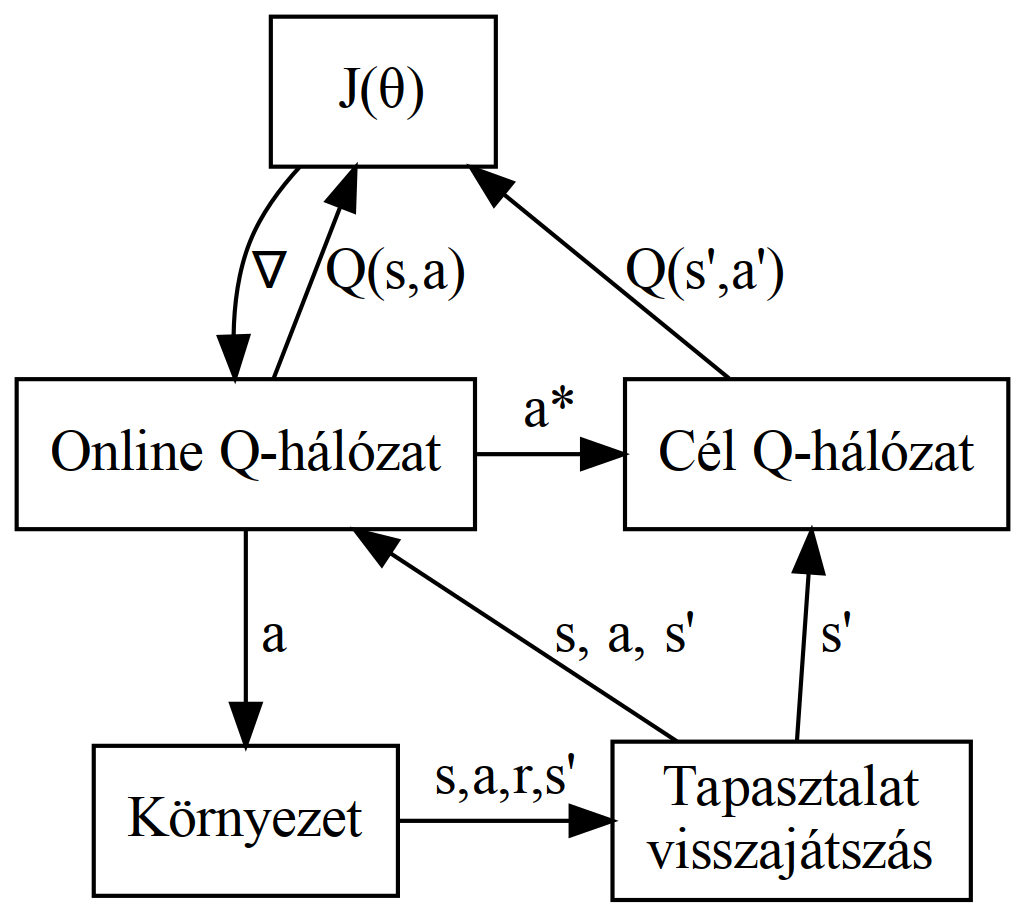
\includegraphics[width=7cm, keepaspectratio]{graphs/dql_2.png}
\end{center}
\end{column}
\end{columns}
\end{frame}

\begin{frame}{A DDQN költségfüggvénye}
\begin{columns}
\begin{column}{.7\textwidth}
A DDQN architektúrában az optimális cselekvés $a^*$ a $Q_\theta$ online hálózat által lesz kiválasztva $s'$ következő állapotra:
\begin{block}{}
\[
a^*=\underset{a'}{argmax}Q_\theta(s',a')
\]
\end{block}
A $Q_{\bar{\theta}}$ célhálózat pedig kiértékeli az online hálózat által választott cselekvést: $Q_{\bar{\theta}}(s',a^*)$, majd kiszámolja a TD hibát: 
\begin{block}{}
\[
J(\theta) = E_{s,a,r,s' \sim D} \left[ \left( r + \gamma Q_{\bar{\theta}}(s',a^*) - Q_\theta(s,a) \right)^2 \right]
\]
\end{block}
Ahol $\{s,a,r,s' \sim D\}$ a tapasztalat visszajátszásból származó miniköteg, $\gamma$ a diszkont ráta. 
\end{column}
\begin{column}{.3\textwidth}
\begin{center}
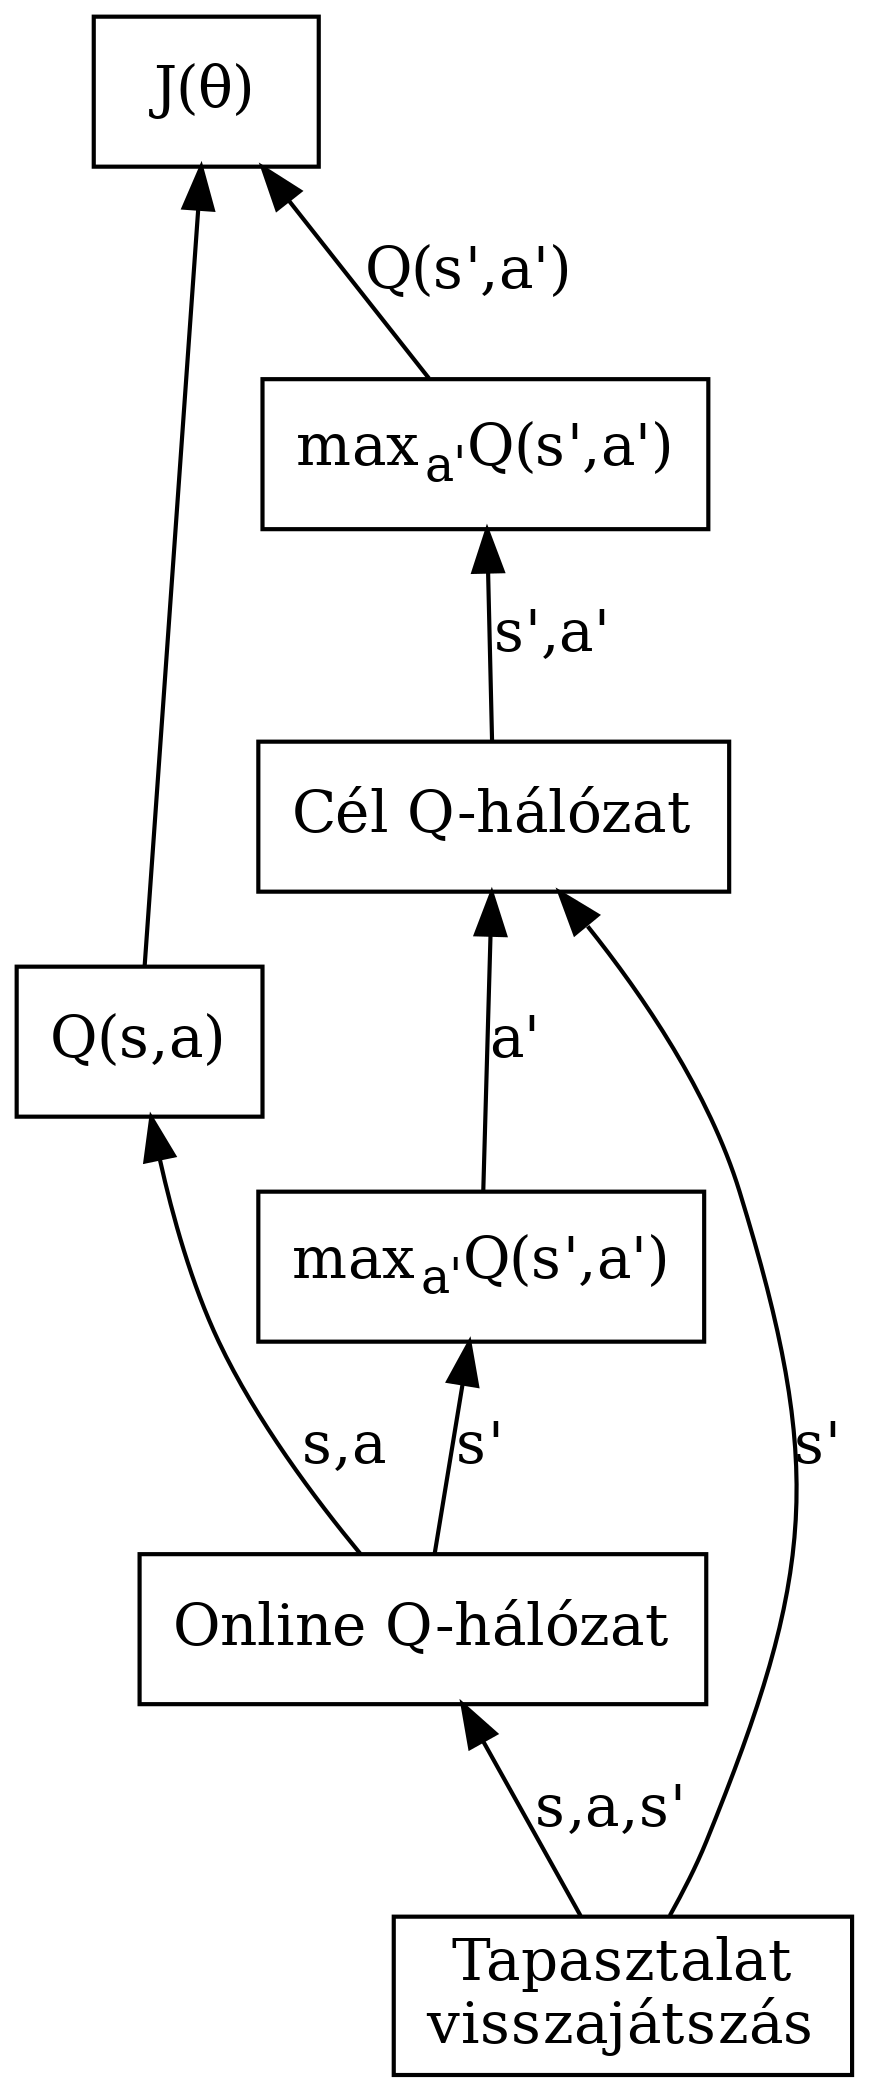
\includegraphics[height=7cm, keepaspectratio]{graphs/dql_3.png}
\end{center}
\end{column}
\end{columns}
\end{frame}

\begin{frame}{A célhálózat frissítése}
\begin{columns}
\begin{column}{.5\textwidth}
Adott időközönként az online hálózat $Q_\theta$ paramétereit át kell másolni a $Q_{\bar{\theta}}$ célhálózatra, \textbf{hiszen a célhálózaton nincs gradiens ereszkedés végrehajtva}.\par\smallskip
Ezt meg lehet tenni úgy is, hogy periodikusan explicit másolat készüljön az online hálózatról, viszont egy jobb megoldás, ha Polyak átlagolással (\textbf{lágy másolással}) másolódnak át a paraméterek.\par\smallskip
\begin{center}
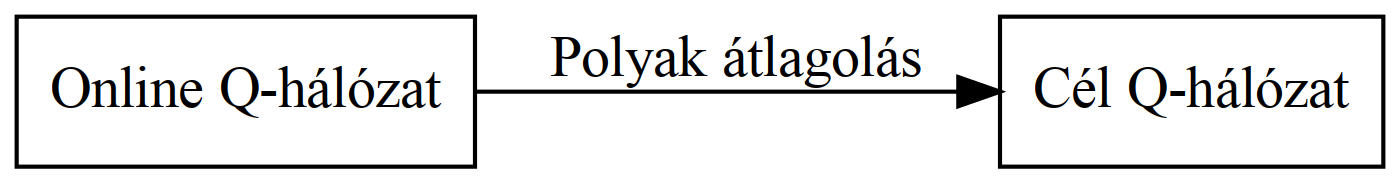
\includegraphics[width=7cm, keepaspectratio]{graphs/dql_4.png}
\end{center}
\end{column}
\begin{column}{.5\textwidth}
Ebben az esetben a $\tau$ hiperparaméter szabályozza az \textbf{átlagolási rátát} vagyis, hogy mekkora súllyal legyenek figyelembe véve az új paraméterek:
\begin{block}{Polyak átlagolás}
\[
\bar{\theta} \leftarrow \tau \theta + (1 - \tau) \bar{\theta}
\]
\vspace{-0.5cm}
\begin{itemize}
	\item $\bar{\theta}$: Célhálózat paraméterei
	\item $\theta$: Online hálózat paraméterei
	\item $\tau$: Átlagolási ráta
\end{itemize}
\end{block}
\end{column}
\end{columns}
\end{frame}

\begin{frame}{}
\begin{algorithm}[H]
\caption{Dupla mély $Q$-tanulás (DDQN)}
\SetAlgoLined
\textbf{Input}: $\tau \sim [0,1]$ átlagolási ráta,
Online hálózat $Q_\theta$, célhálózat $Q_{\bar{\theta}}$, tapasztalat memória $D$ inicializálása\;
\For{$i = 0 \rightarrow max_i$}{
	\For{$t = 0 \rightarrow max_t$}{
		$s$ megfigyelése és $a \sim \pi(s,a)$ cselekvés választása\;
		$a$ végrehajtása és $s'$, $r$ megfigyelése\;
		$s, a, r, s'$ eltárolása a tapasztalat memóriában\;
	}
	\For{$c = 0 \rightarrow max_c$}{
		$e = s, a, r, s' \sim D$\tcc*[t]{Mintavétel a tapasztalat memóriából}
		$Q^*(s,a) \leftarrow r + \gamma Q_\theta(s', argmax_{a'}Q_{\bar{\theta}}(s',a'))$\;
		Gradiens ereszkedés végrehajtása a $(Q^*(s,a) - Q_\theta(s,a))^2$ hibán\;
		$\bar{\theta} \leftarrow \tau \theta + (1 - \tau) \bar{\theta}$\tcc*[t]{Paraméterek frissítése}
	}		
}
\end{algorithm}
\end{frame}

\section{Párbajozó mély $Q$-tanulás}

\begin{frame}
\tableofcontents[currentsection]
\end{frame}

\begin{frame}{Az előny függvény}
A megerősítéses tanulás harmadik értékfüggvénye a $V(s)$ és a $Q(s,a)$ mellett.\par\smallskip
Matematikailag az előny függvény $s$ állapotra és $a$ cselekvésre a cselekvés $Q(s,a)$ minőségének és $s$ állapot $V(s)$ értékének a különbsége:
\begin{block}{Előny függvény}
Az előny függvény megadja, \textbf{mennyivel jobb vagy rosszabb} egy adott $a$ cselekvést végrehajtani egy $s$ állapotból a többi elérhető cselekvéshez képest.
\[
A(s,a) = Q(s,a) - V(s)
\]
Egy $A(s,a)=0$ érték azt jelenti, hogy $a$ cselekvést végrehajtani olyan jövedelmező, mint az átlagos cselekvés $s$-ből. Ha $A(s,a)>0$, a cselekvés jobb, és ha $A(s,a)<0$ akkor rosszabb mint az átlagos cselekvés $s$ állapotból.
\end{block}
\end{frame}

\begin{frame}{Párbajozó $Q$-hálózat architektúrája}
\begin{columns}
\begin{column}{.6\textwidth}
\only<1>{A párbajozó $Q$-tanulás algoritmusa \textbf{explicit módon kettéválasztja az állapot-érték és előny függvények megbecslését} minden állapot művelet esetén. Ez a szétválasztás teszi lehetővé a hatékonyabb tanulást és jobb általánosítást.\par\smallskip
Az előnyfüggvény definíciójából kiindulva a minőségfüggvényt ki lehetne számolni úgy, mint $Q(s,a)=V(s)+A(s,a)$, \textbf{viszont ez problémás mert nem feltételezhető, hogy a hálózat minden értékre pontos becslést ad}.\par\smallskip}
\only<2>{A gyakorlatban a $Q(s,a)$ érték úgy áll elő, hogy a $V(s)$ állapot-értékhez hozzáadódik a választott cselekvés előnyének és az összes cselekvés átlagos előnyének különbsége:
\begin{block}{}
\vspace{-0.5cm}
\[
Q(s,a) = V(s) + \left( A(s,a) - \frac{1}{\vert A \vert} \sum_{a'} A(s,a') \right)
\]
\end{block}
Ahol $\vert A \vert$ az elérhető cselekvések száma, $\frac{1}{\vert A \vert} \sum_{a'} A(s,a')$ pedig az elérhető cselekvések előnyeinek átlaga.}
\end{column}
\begin{column}{.4\textwidth}
\begin{center}
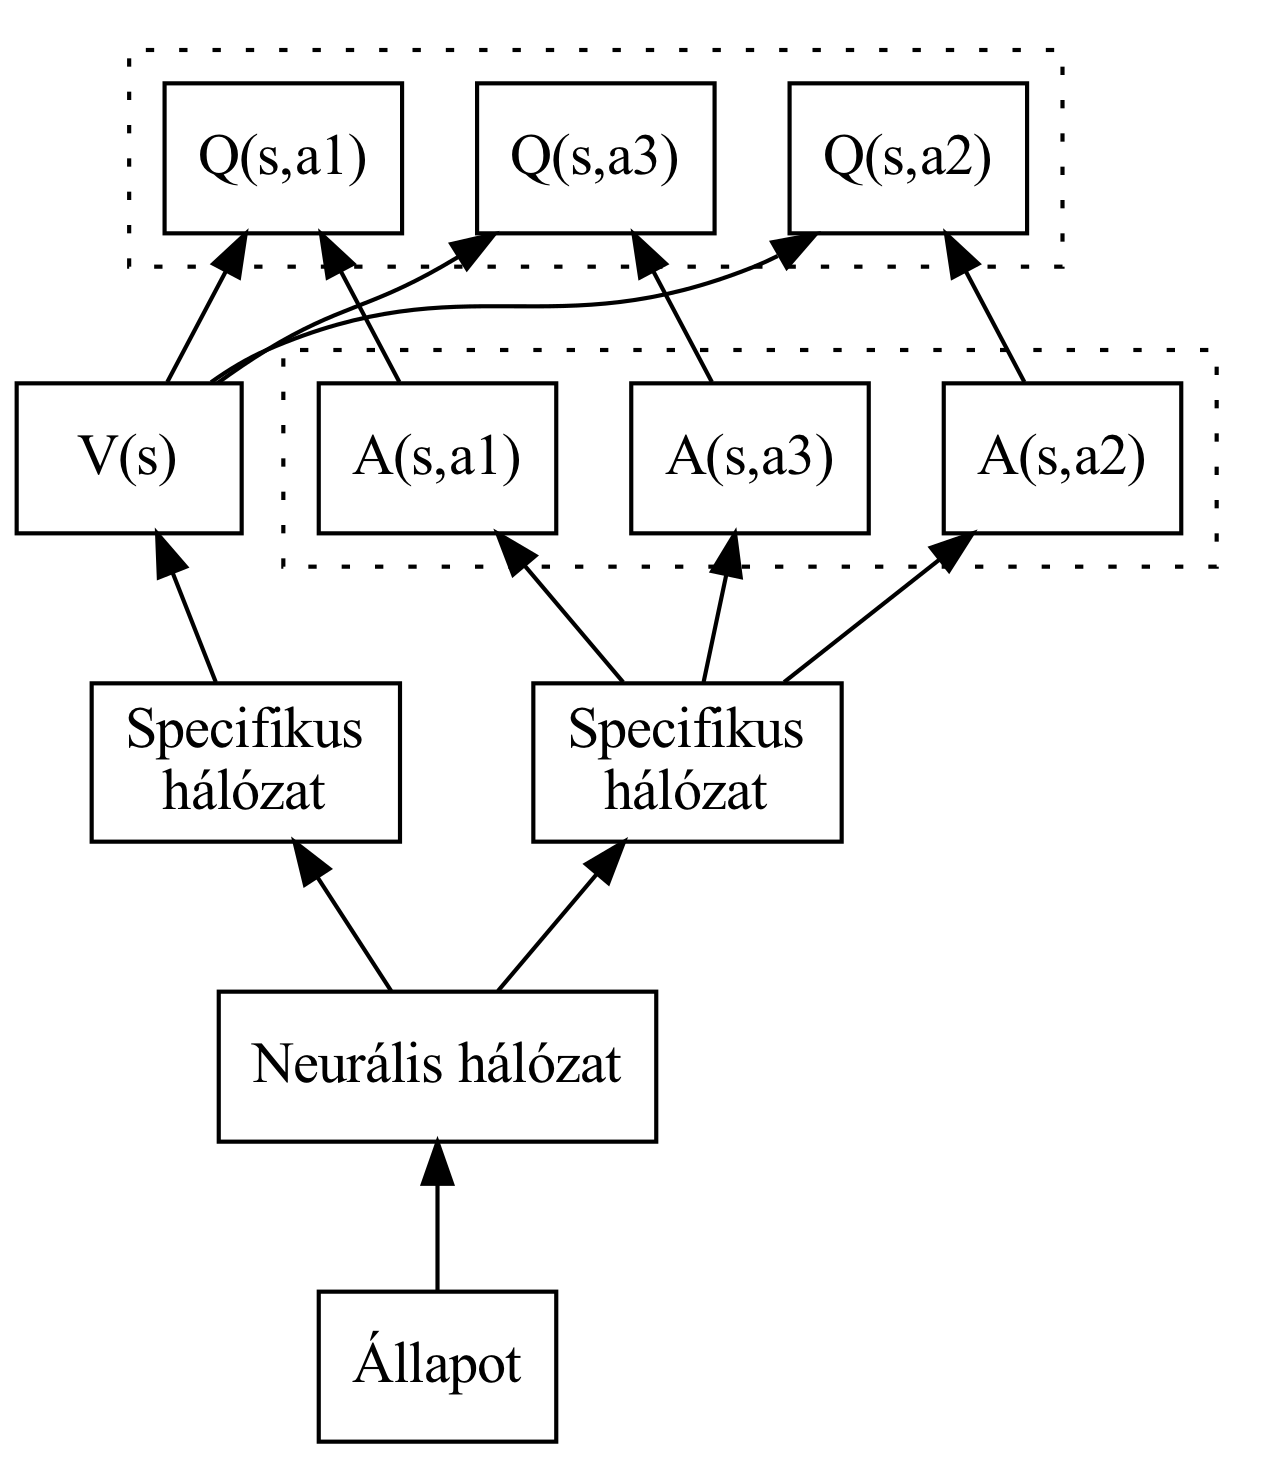
\includegraphics[height=6.5cm, keepaspectratio]{graphs/dql_5.png}
\end{center}
\end{column}
\end{columns}
\end{frame}

\begin{frame}{Az egycsatornás és párbajozó architektúrák összehasonlítása}
\begin{center}
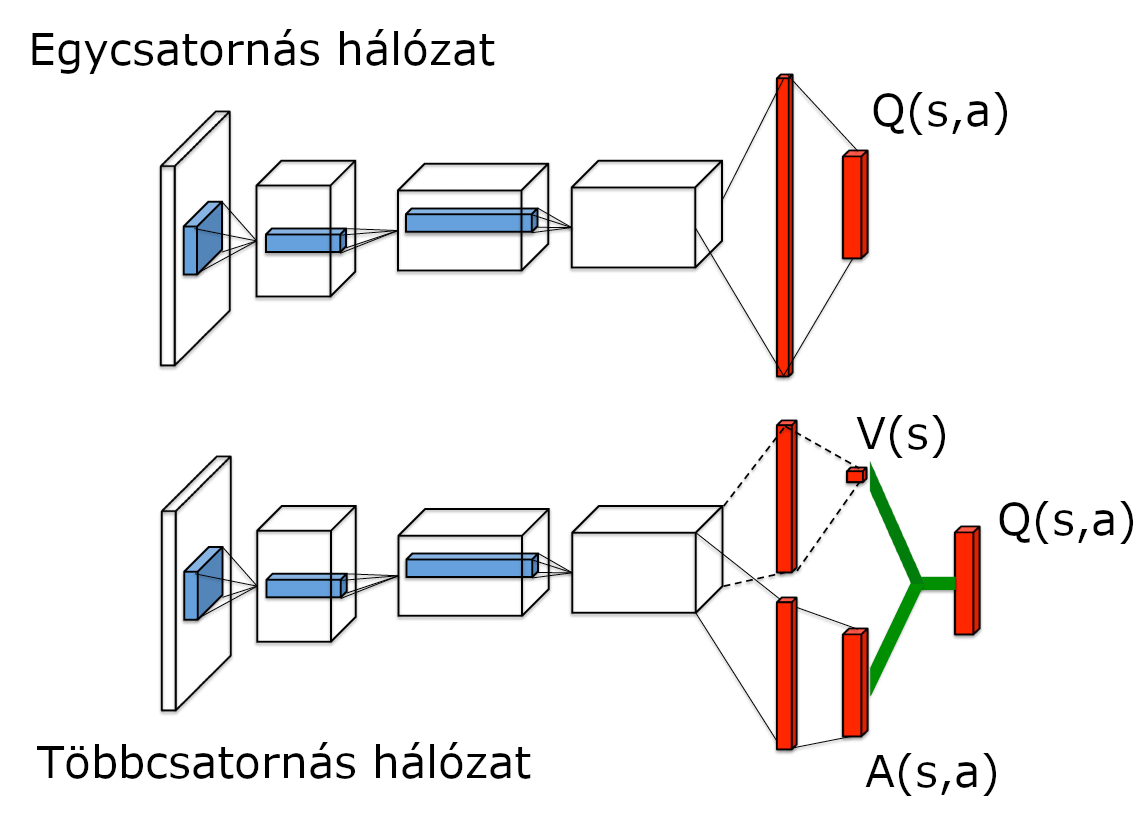
\includegraphics[width=10cm, keepaspectratio]{images/dql_2.png}
\end{center}
\end{frame}

\begin{frame}{Dupla párbajozó architektúrák (DDDQN)}
\begin{columns}
\begin{column}{.5\textwidth}
A kettős $Q$-tanulást meg lehet valósítani párbajozó hálózatokkal is. Mivel mindkettőnek az outputja a $Q(s,a)$ állapot-cselekvés minőség függvény, \textbf{az egyetlen változtatás a kettős $Q$-tanuláshoz képest a neurális hálózat architektúrájában van}. A komponensek elrendezésén nem szükséges módosítani.\par\smallskip
A hálózatok között a paraméterek másolását explicit másolással, vagy Polyak átlagolással lehet megoldani. Ezzel a hálózat pontosabban tanul, és ellenállóbb a tanítási mintában jelen lévő zajjal szemben.
\end{column}
\begin{column}{.5\textwidth}
\begin{center}
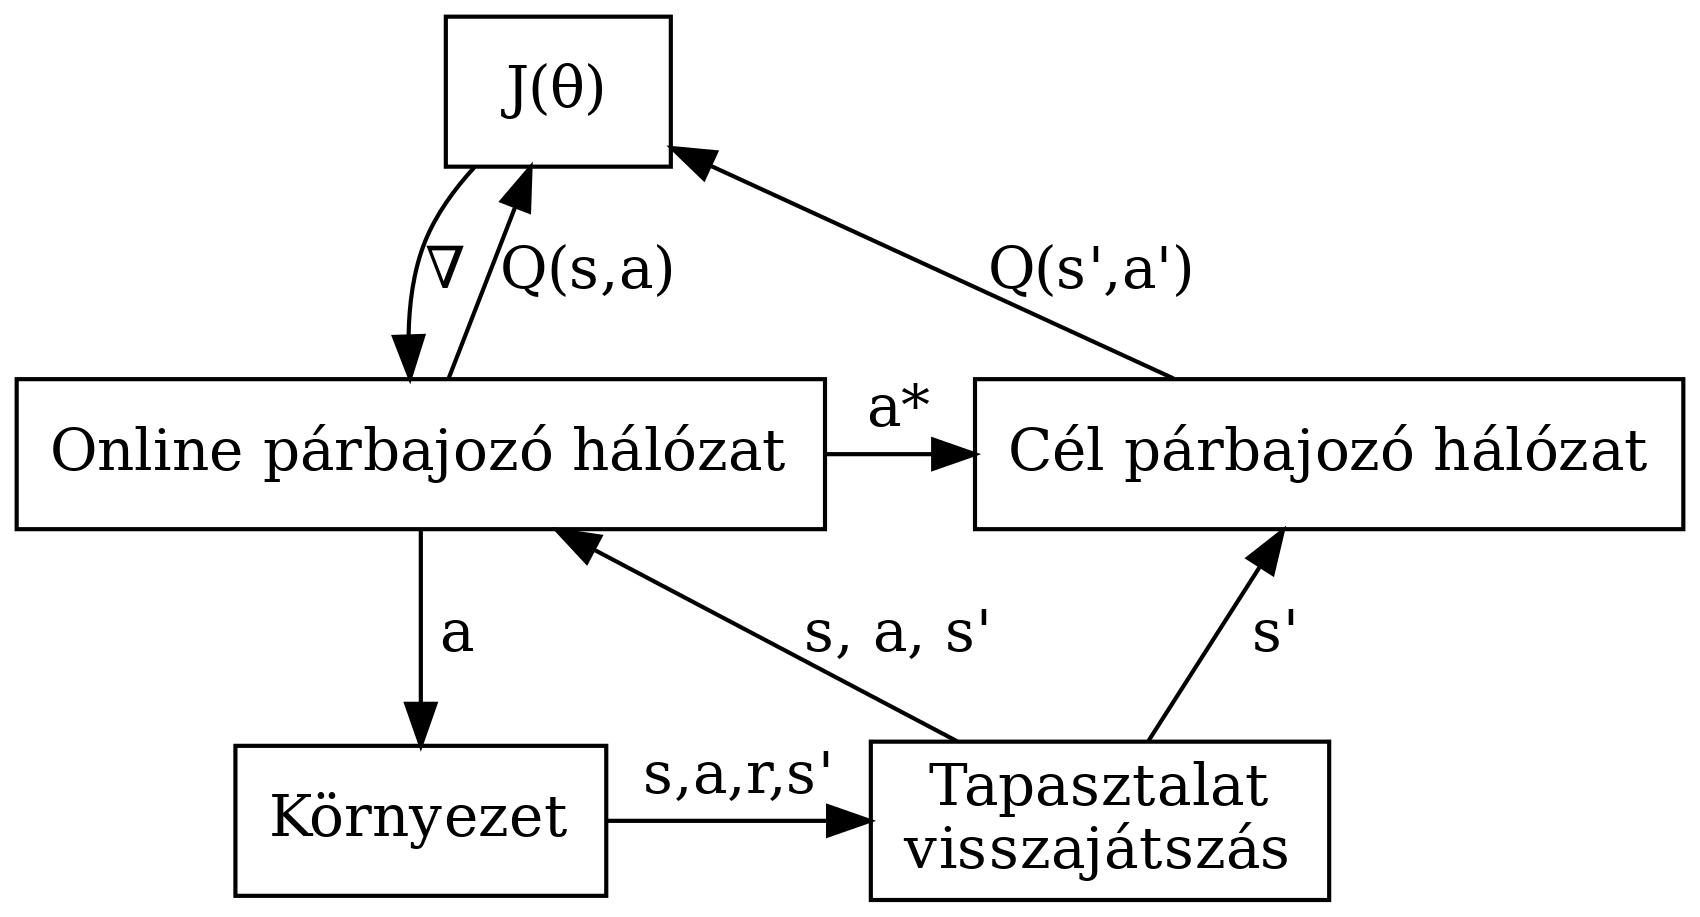
\includegraphics[width=7.5cm, keepaspectratio]{graphs/dql_6.png}
\end{center}
\end{column}
\end{columns}
\end{frame}

\section{Aktor-kritikus}

\begin{frame}
\tableofcontents[currentsection]
\end{frame}

\begin{frame}{Aktor-kritikus architektúra}
\begin{columns}
\begin{column}{.6\textwidth}
Az aktor-kritikus architektúra egy kettős tanulási eljárás, amely kombinálja a politikaalapú (\textbf{aktor}) és az értékalapú (\textbf{kritikus}) eljárásokat a tanítási folyamat javítása és a gyorsabb konvergencia érdekében.\par\smallskip
\begin{itemize}
	\item \textbf{Aktor}: Az állapothoz tartozó cselekvés kiválasztásáért felel. Egy politikát tanul meg, ami az állapotokhoz cselekvéseket rendel. Célja, hogy maximalizálja a várható kumulált hozamot. 
	\item \textbf{Kritikus}: Feladata megbecsülni a $V(s)$ állapot-érték függvényt. A kritikus segíti az aktort azzal, hogy visszajelzést ad neki az általa megtett cselekvések minőségéről. 
\end{itemize}
\end{column}
\begin{column}{.4\textwidth}
\begin{center}
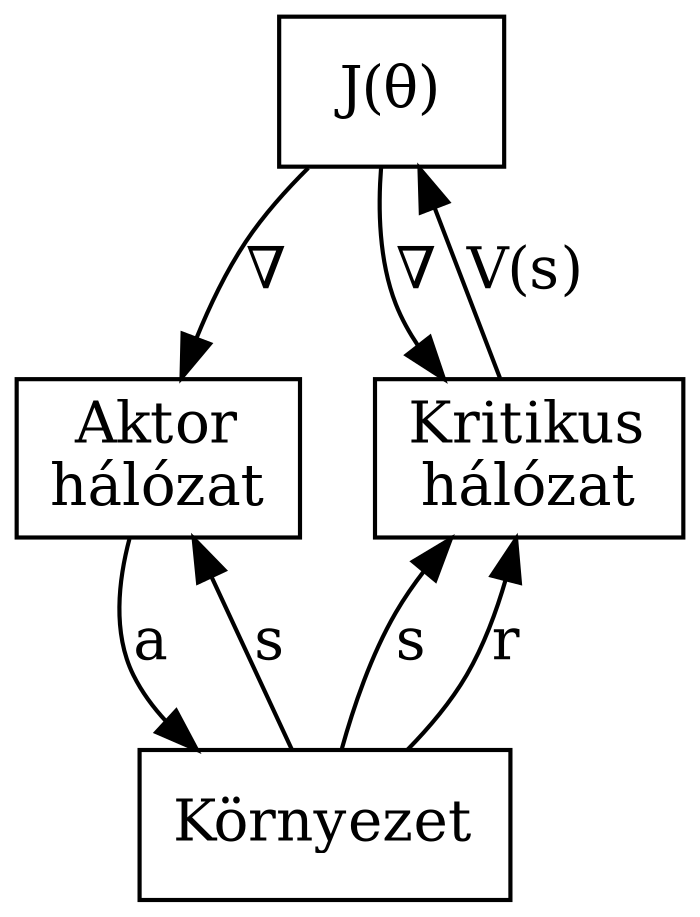
\includegraphics[height=6cm, keepaspectratio]{graphs/dql_7.png}
\end{center}
\end{column}
\end{columns}
\end{frame}

\begin{frame}{Az aktor-kritikus költségfüggvény}
\begin{columns}
\begin{column}{.5\textwidth}
Az előnyalapú aktor-kritikus eljárásokban az aktor az $A(s,a)$ előnyfüggvényt becsüli meg a saját neurális fejében. A kritikus pedig egy logaritmikus valószínűségi eloszlást.
\begin{block}{Az AAC költségfüggvénye}
\[
J(\theta) = \sum_{t=0}^{T-1} log \pi_\theta (a \vert s) A(s,a)
\]
Ahol $\pi_\theta (a \vert s)$ az a valószínűség, hogy a $\pi_\theta$ szerint mekkora valószínűséggel hajtja végre az ügynök $a$ cselekvést $s$ állapotból, és $A(s,a)$ az előnyfüggvény.
\end{block}
\end{column}
\begin{column}{.5\textwidth}
\begin{center}
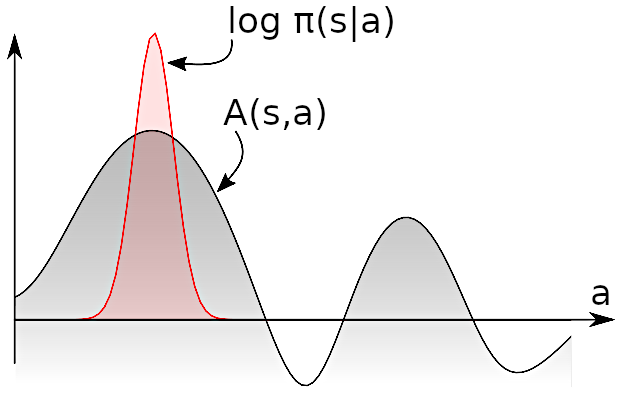
\includegraphics[width=7cm, keepaspectratio]{images/dql_3.png}
\end{center}
\end{column}
\end{columns}
\end{frame}

\begin{frame}{A modellezés folyamata}
\begin{enumerate}
	\item \textbf{Inicializáció}: Az aktor és kritikus hálózatok kezdősúlyainak megadása: $\theta$, $\phi$, tanulási sebesség beállítása: $\alpha$
	\item \textbf{Tapasztalat gyűjtése}: az aktor interakcióba lép a környezettel
	\item \textbf{Előny kiszámítása}: $A(s,a) = (V(s) - (r + V(s')))^2$ megadja, hogy egy adott $a$ cselekvés mennyire jövedelmező a többihez képest
	\item \textbf{Aktor frissítése}: gradiens ereszkedés a $log \pi_\theta (a \vert s) A(s,a)$ előny értéken
	\item \textbf{Kritikus frissítése}: gradiens ereszkedés a $(V(s) - (r + V(s')))^2$ hibán
	\item \textbf{Iteráció} folytatása a kilépésig
\end{enumerate}
\end{frame}

\begin{frame}
\begin{algorithm}[H]
\caption{Előnyalapú aktor-kritikus tanítás}
\SetAlgoLined
Aktor $\pi_\theta(s)$ és kritikus $V_\phi(s)$ inicializálása\;
\For{$i = 0 \rightarrow max_i$}{
	$s$ inicializálása a kezdőállapottal\;
	\While{$s \neq s_T$}{
		$a \leftarrow \pi_\theta(s)$\tcc*[t]{Az aktor cselekvést választ}
		$a$ végrehajtása a környezetben, $r$ és $s'$ megfigyelése\;		
		$A(s,a) \leftarrow r + \gamma V_\phi(s') - V_\phi(s)$\tcc*[t]{Előny kiszámítása}
		$\theta \leftarrow \theta + \alpha \nabla log \pi_\theta (a \vert s) A(s, a)$\tcc*[t]{Aktor frissítése}
		$\phi \leftarrow \phi + \alpha \nabla A(s,a)^2$\tcc*[t]{Kritikus frissítése}
	}
}
\end{algorithm}
Ahol $\theta$ az aktor, és $\phi$ a kritikus paraméterlistája.
\end{frame}

\end{document}











